    \section{Motivation}
    Um die Einflüsse verschiedener Kurzschlussanordnungen und -ausführungen schon im Vorfeld abschätzen zu können und ein erstes Gefühl für den Einfluss der Kurzschlüsse zu bekommen, wurde die Testanordnung zunächst ausgiebig mit der Simulationssoftware CST simuliert.\\
    Die Simulationen dienten als Vorbereitung, um bei den Messungen präziser vorgehen zu können und gezielt Messungen durchzuführen. Zuletzt wurden die Simulationsergebnisse dann mit den Messergebnissen gegenübergestellt und verglichen, um deren Richtigkeit zu überprüfen.
    
    \section{Modellierung}
        \subsection{Bestehendes Testbox- und Ringkernmodell}
        Als Grundlage für die Simulation der Testbox und des Ringkerns dient das Simulationsmodell von Testbox inklusive Ringkern aus der Bachelorarbeit von Denys Bast \cite{bast2017ba}.\\
        Die Außenwände der Testbox sind geometrisch sehr genau den Abmessungen des realen Teststandes entsprechend modelliert, als Material wird hierfür reines Kupfer verwendet, wie es in der Datenbank von CST zu finden ist. Die leere Box ist in Abbildung~\ref{fig:BoxCST} dargestellt.
        
            \begin{figure}[htb]
                \centering
                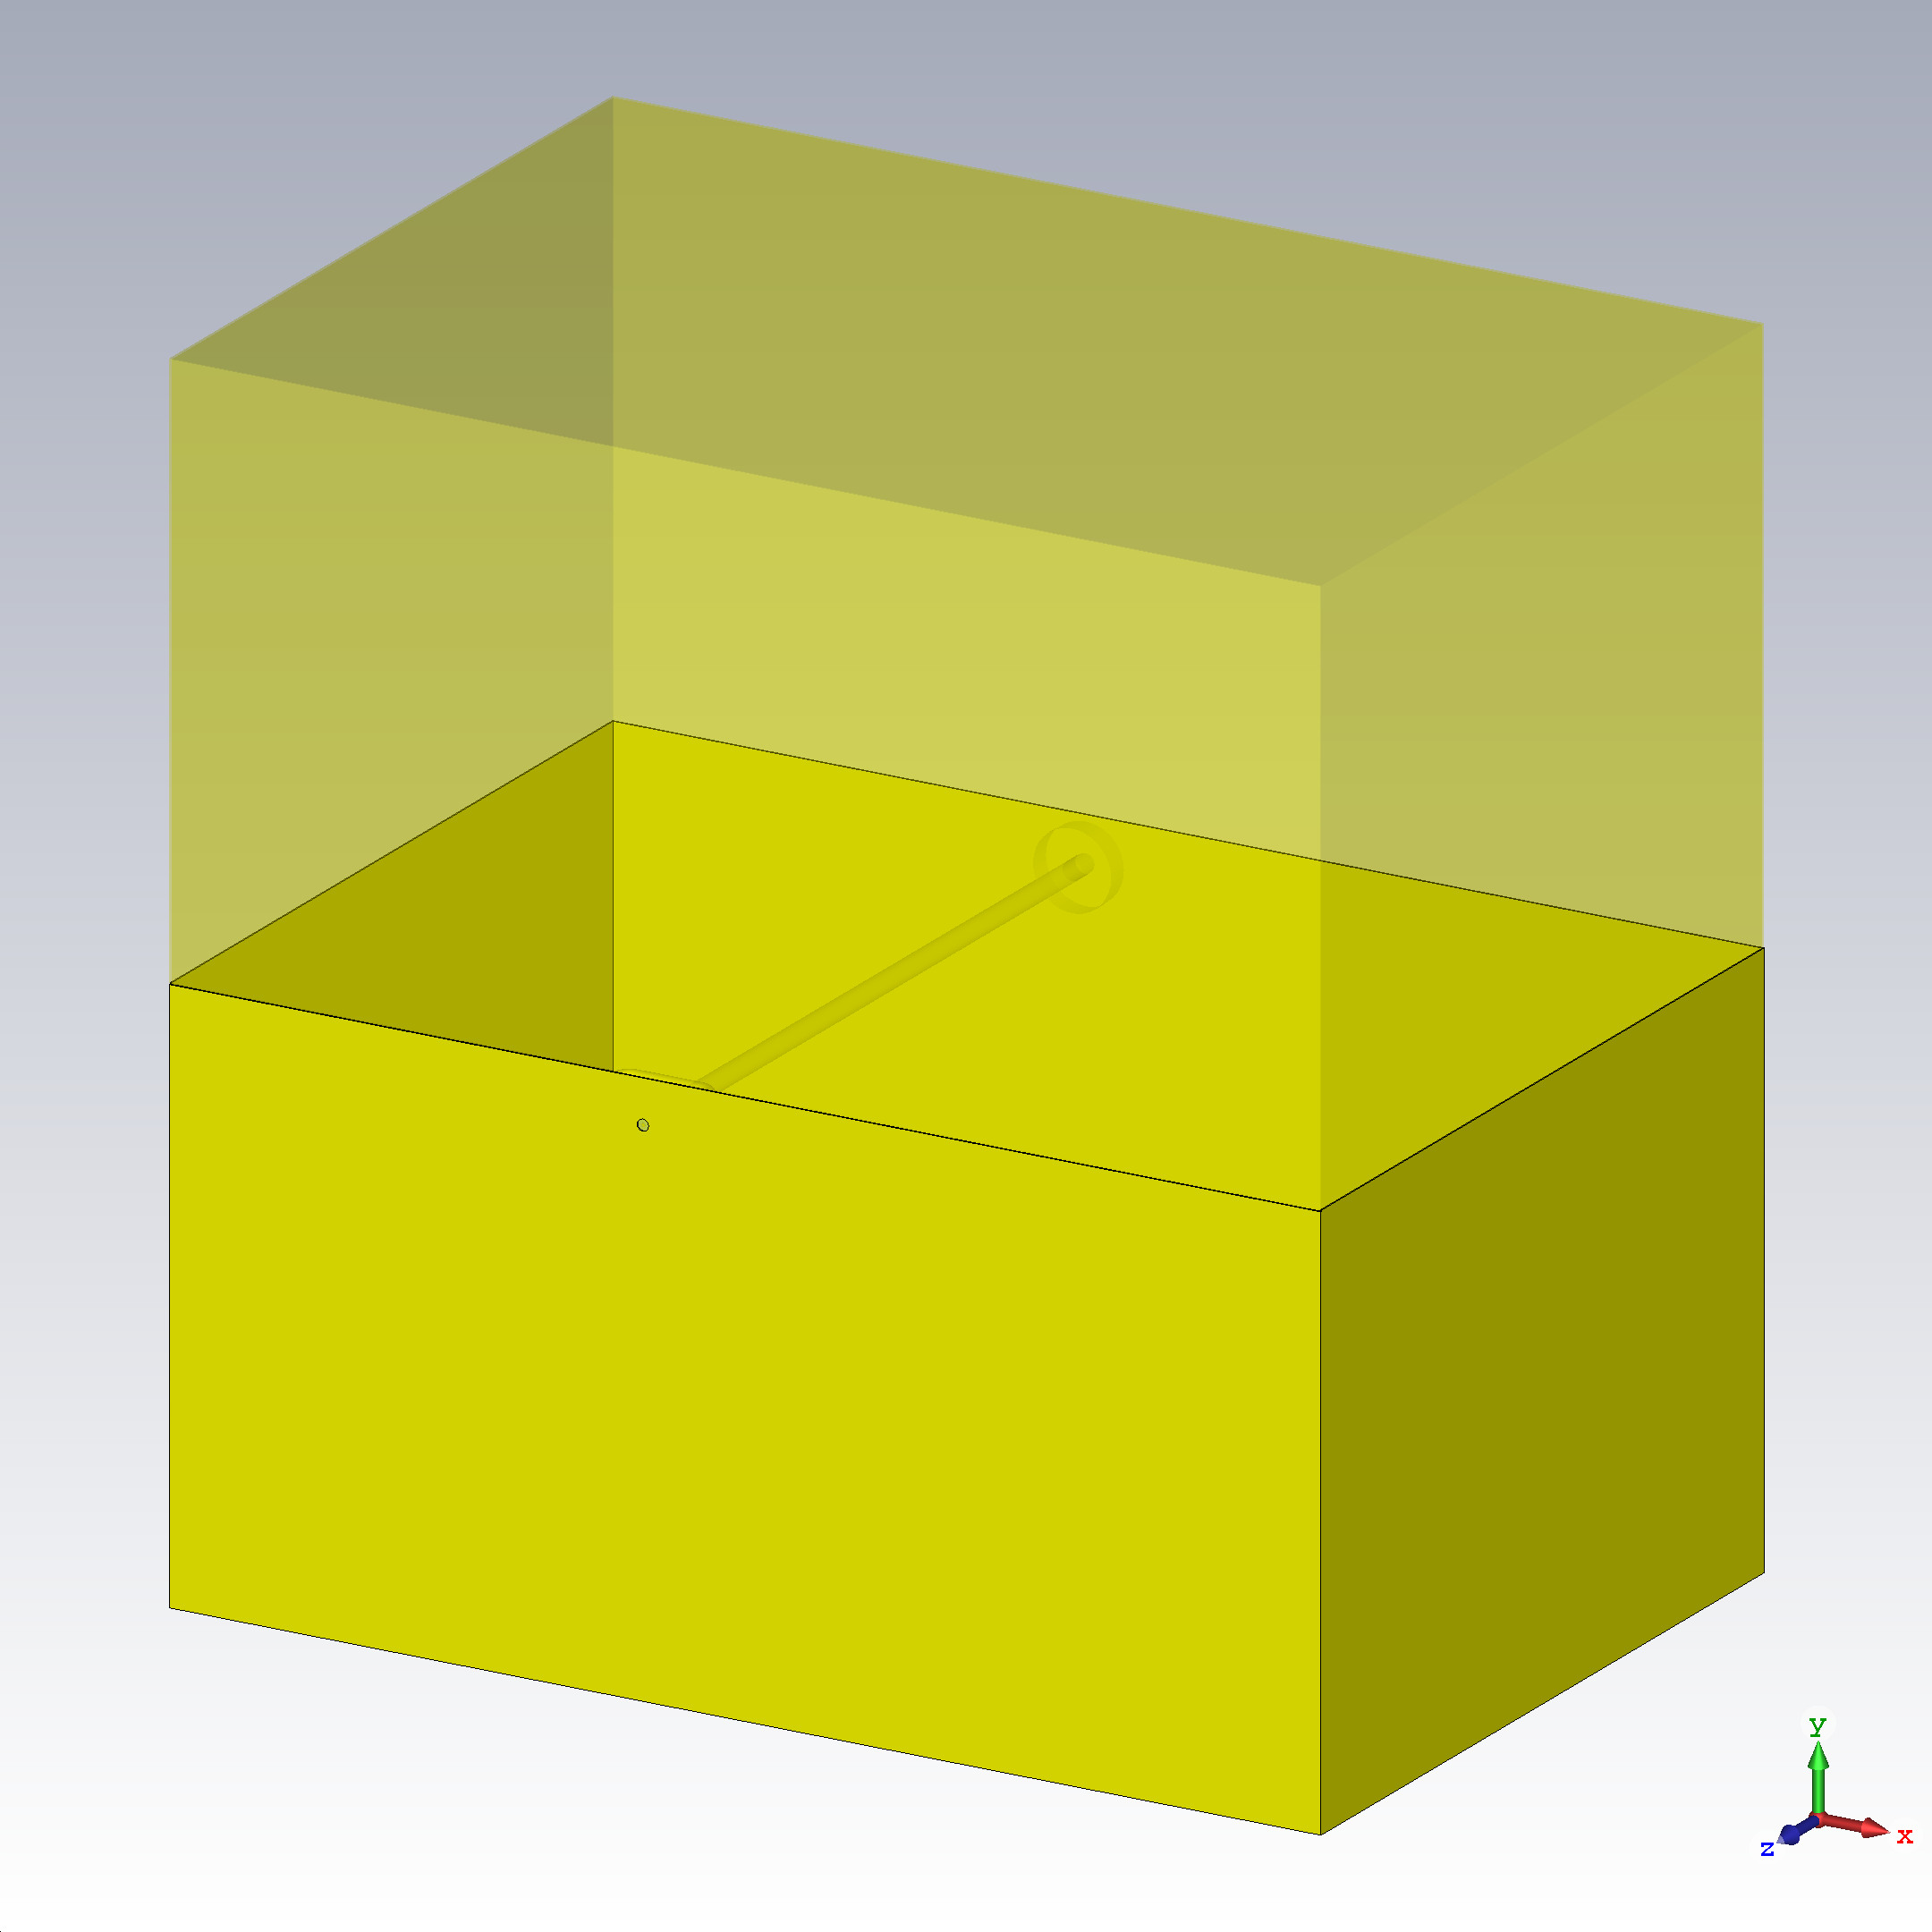
\includegraphics[height=0.4\textwidth]{./Simulation/BoxWaende2.png}
                \caption{Modell der Testbox in CST}
                \label{fig:BoxCST}
            \end{figure}
        In Abbildung~\ref{fig:InnenleiterCST} ist die Signaleinkopplung der Testbox zu sehen.
        Diese ist als Hohlzylinder aus Kupfer modelliert und geometrisch genau am realen Vorbild orientiert. Die Stange ist an der hinteren Wand elektrisch mit der Box verbunden und an der Vorderseite durch einen elektrisch nicht leitfähigen Ring aus Polyethylen (PE, CST Datenbank) von der Box isoliert. Hierdurch wird erreicht, dass die Stange als Hin- und die Boxaußenwände als Rückleiter für Signale dienen. Der Übergang zwischen Testbox, PE und Stange ist planar ausgeführt, um einen Signalport für die Simulation darzustellen.
        
            \begin{figure}[htb]
                \centering
                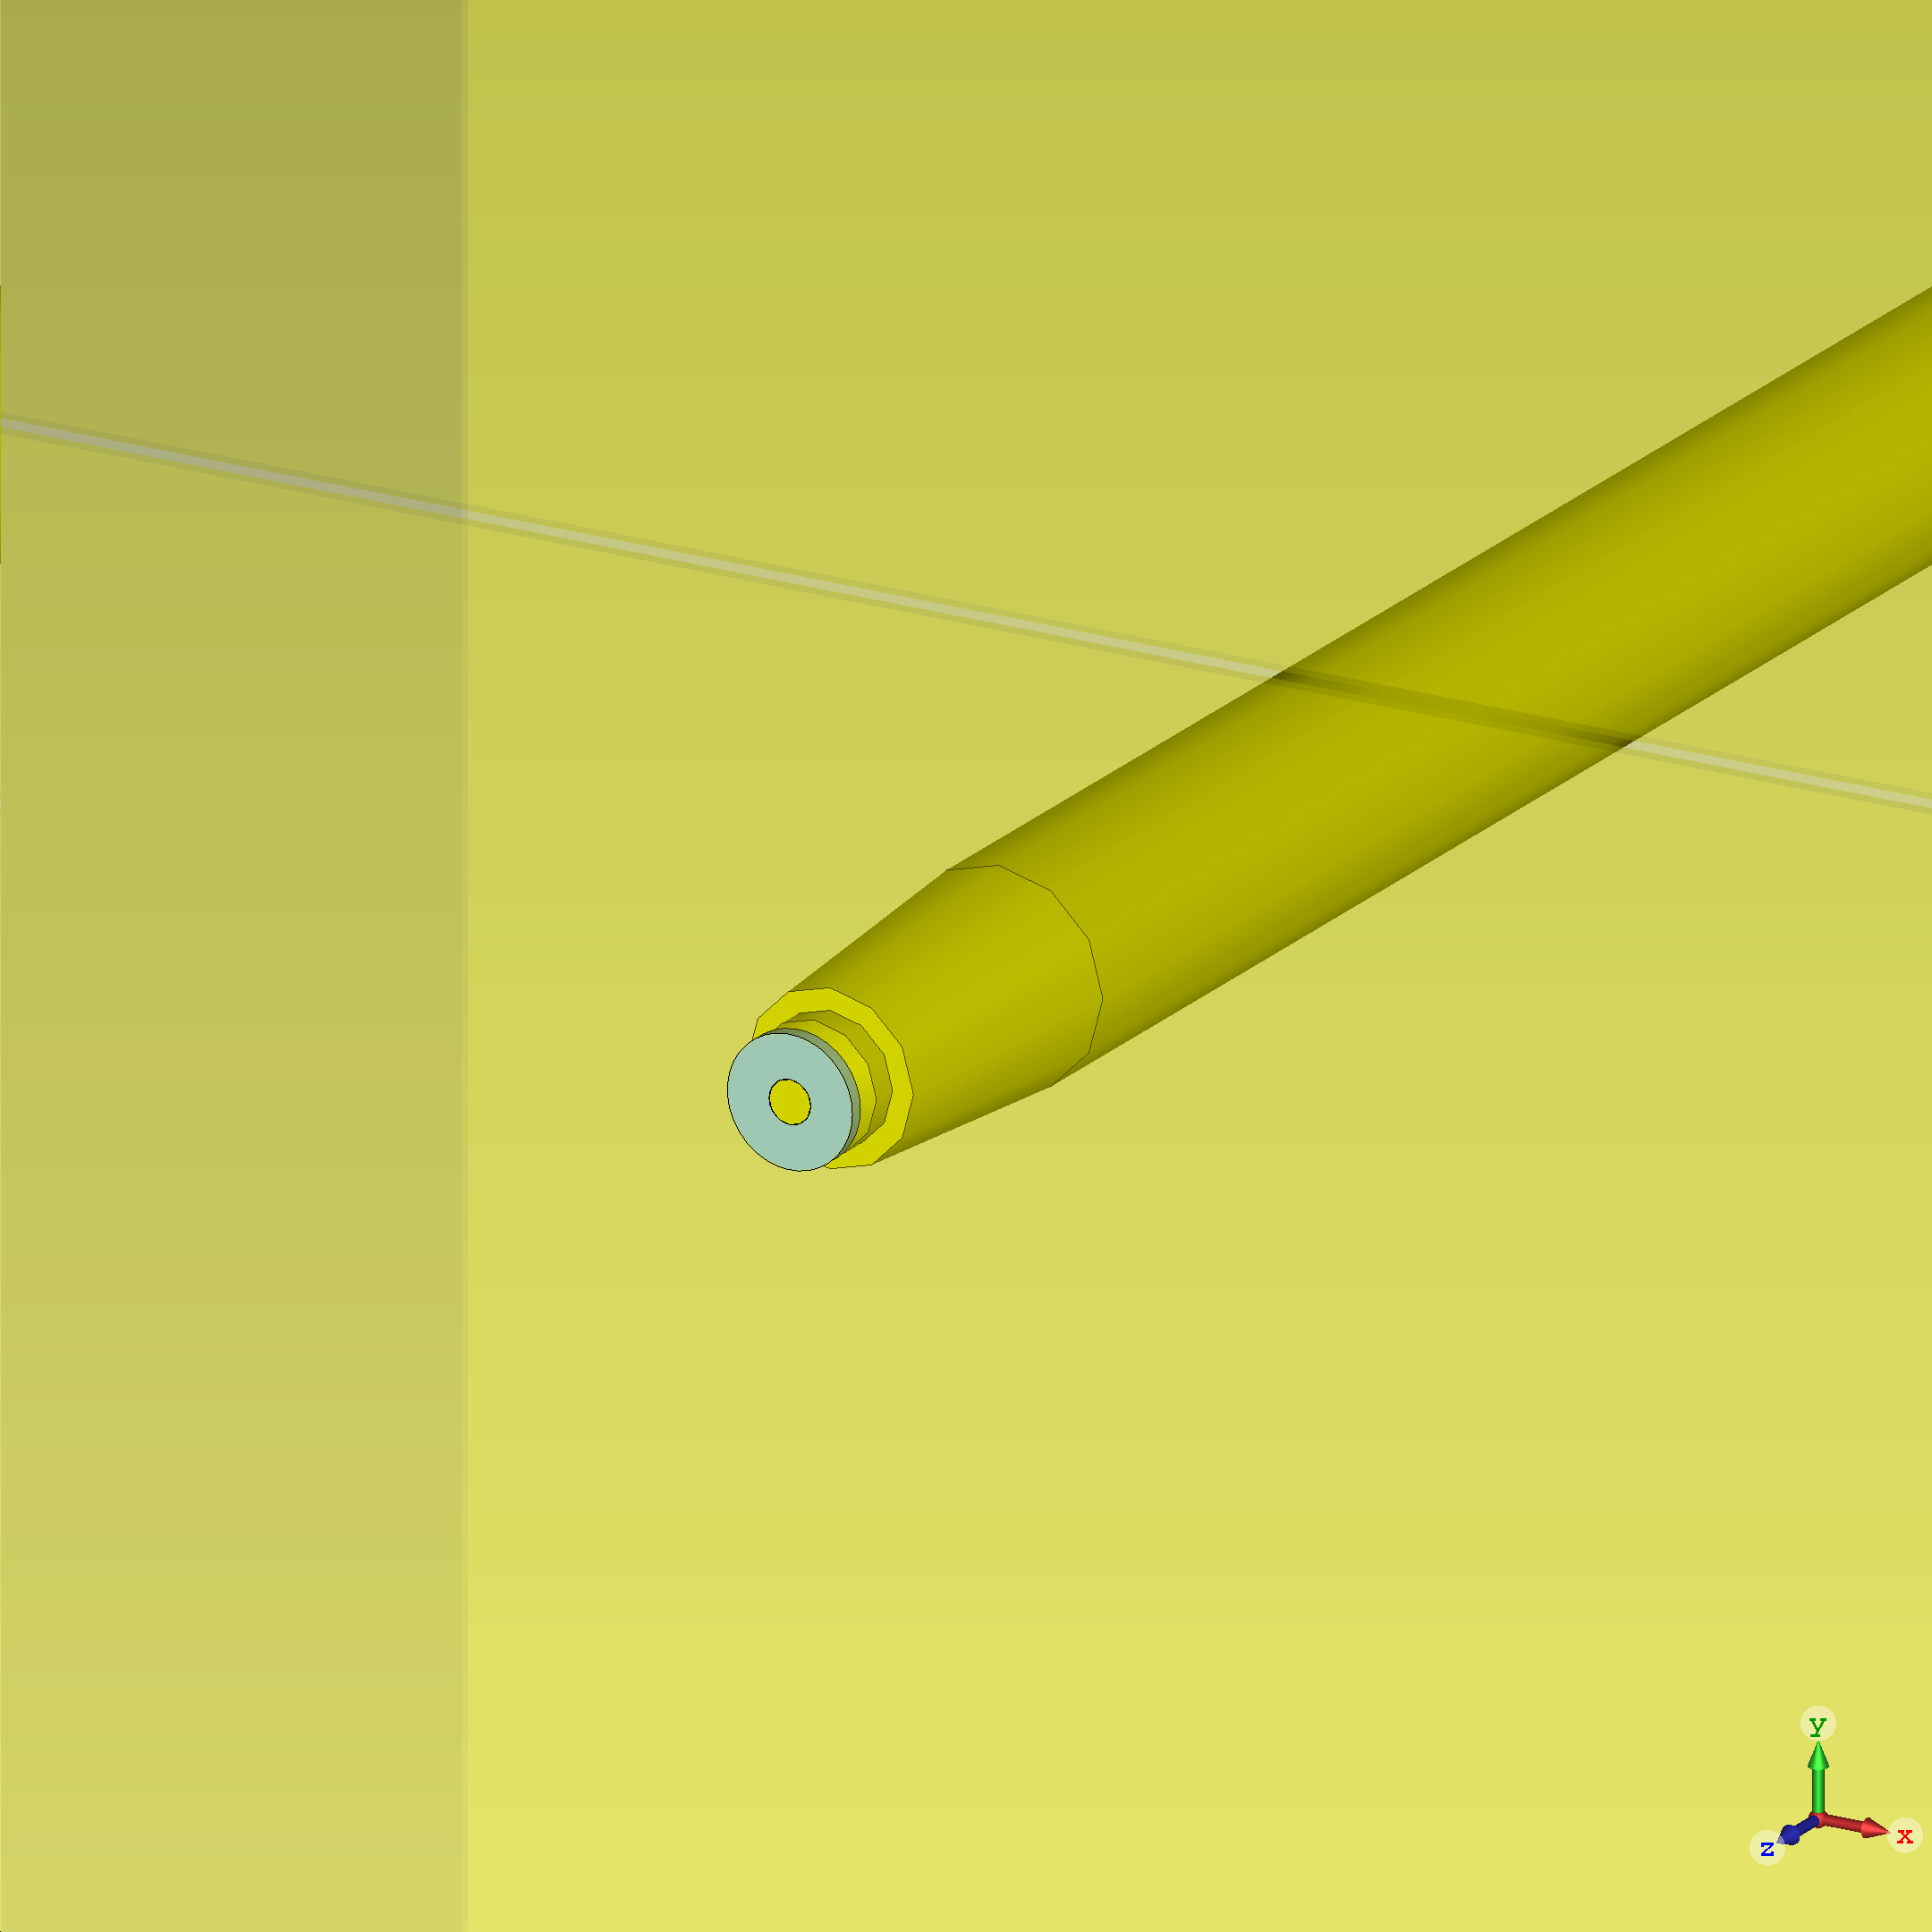
\includegraphics[height=0.4\textwidth]{./Simulation/InnenleiterPE.png}
                \caption{Modell der Einkopplungsstange mit elektrischer Isolation}
                \label{fig:InnenleiterCST}
            \end{figure}
        
        Der Ringkern ist als einfacher Hohlzylinder mit den geometrischen Abmessungen seines realen Vorbild modelliert. Der realem Aufbau entsprechend, ist er zentral im Testboxmodell, allerdings freischwebend, ohne die hölzerne Halterung, modelliert.\\
        Ein grundlegender Aspekt der Arbeit von Denys Bast~\cite{bast2017ba} ist, die magnetische Permeabilität des Ringkernmaterials in der Simulation mit dem realen Material in Übereinstimmung zu bringen. Die dabei gewonnenen Daten wurden übernommen.
        
            \begin{figure}[htb]
                \centering
                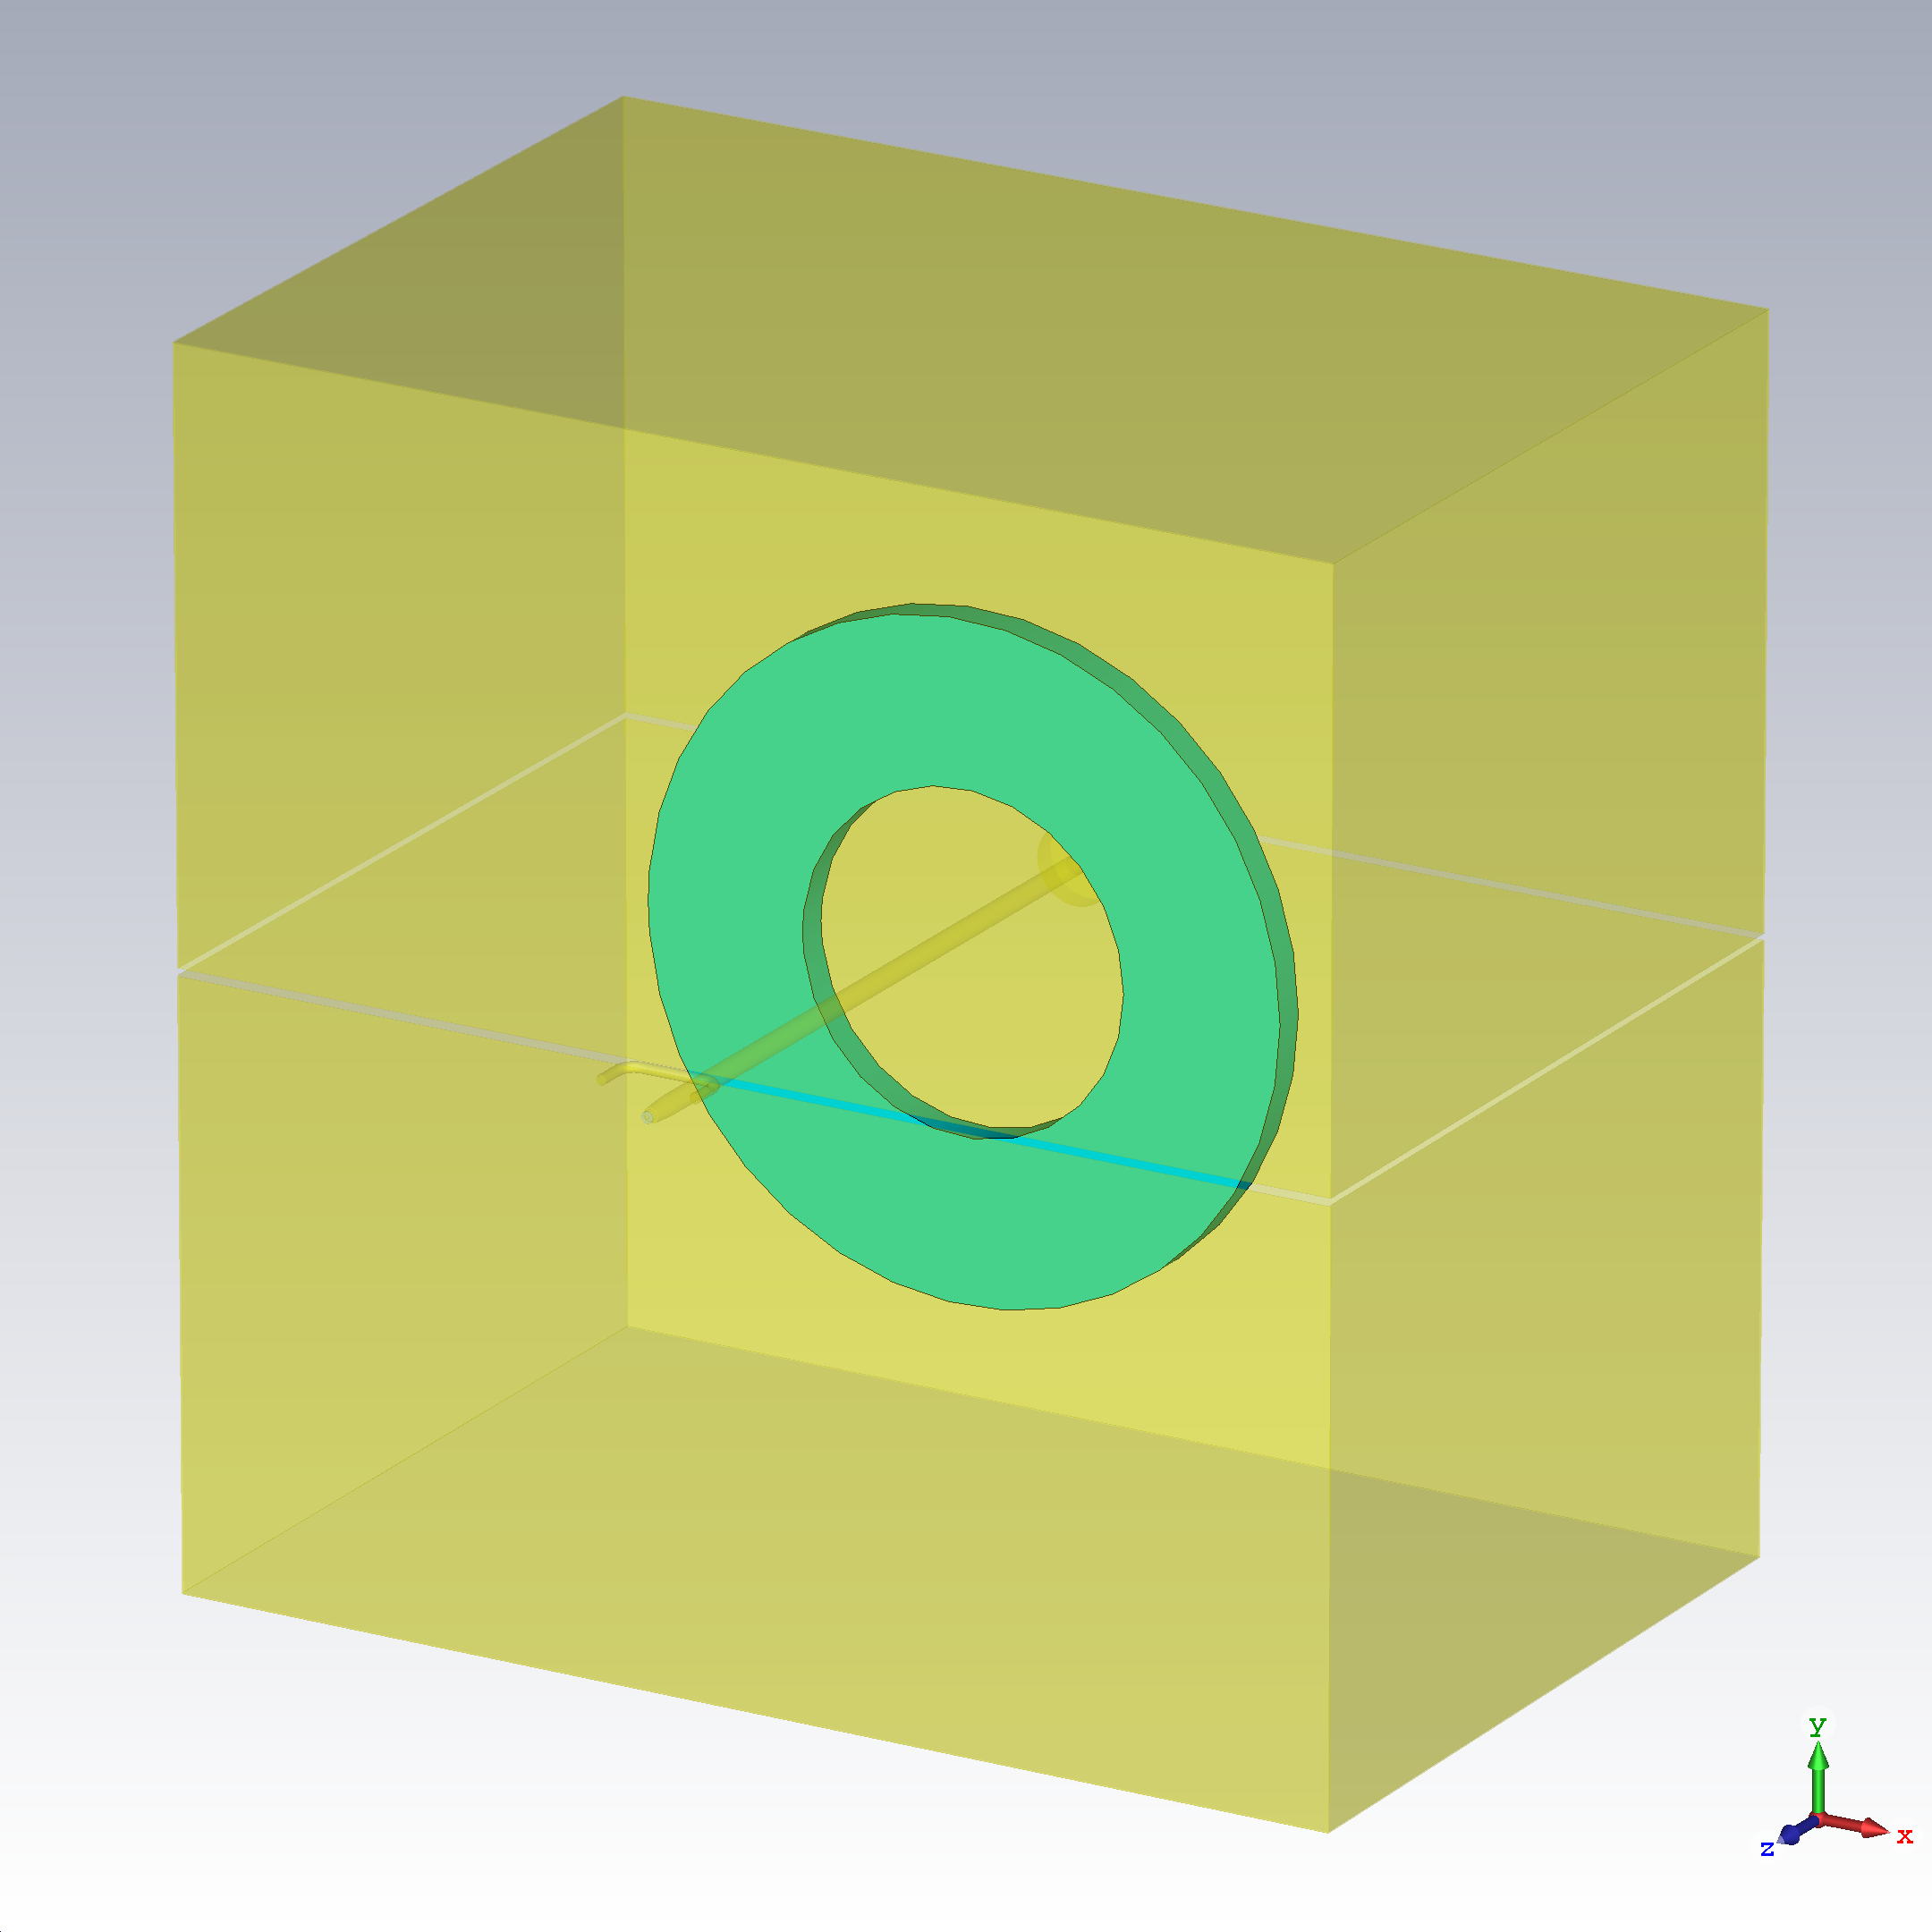
\includegraphics[height=0.4\textwidth]{./Simulation/BoxRK.png}
                \caption{Gesamtdarstellung der Modellierung von Testbox und Ringkern nach Denys Bast~\cite{bast2017ba}}
                \label{fig:BoxRKCST}
            \end{figure}
        
        Abbildung~\ref{fig:BoxRKCST} bildet den modellierten Aufbau der Testbox mit Ringkern ab, wie er in \cite{bast2017ba} beschrieben wird.

        \subsection{Kurzschlüsse}
        Die für die Parameteranalyse dieser Arbeit benötigten Kurzschlüsse sind in CST in verschiedenen, komplexen Ausführungen modelliert.\\
        Die erste Version stellt ein einfacher, ellipsenförmiger Torus dar, wie er in Abbildung~\ref{fig:KSCST}\subref{subfig:V1} abgebildet ist. Als Material für die Simulation wird Kupfer aus der Datenbank von CST verwendet.\\
        Die in Kapitel~\ref{sec:testbox} beschriebenen Verbesserungen der Kurzschlüsse für eine erhöhte Reproduzierbarkeit der Messungen, sind so in CST modelliert. Abbildung~\ref{fig:KSCST}\subref{subfig:V2} zeigt die Umformung des einfachen Torus zu einem schienenförmigen Kurzschluss. Die finale Version, die letztlich für die Messungen benutzt wurde, ist in Abbildung~\ref{fig:KSCST}\subref{subfig:V3} zu sehen. Die einfache Kupferschiene ist geometrisch an die verwendeten Kurzschlüsse angepasst und um die Verbindungsschrauben erweitert.
        
            \begin{figure}[htb]
                \centering
                \subfloat[Version 1]{
                    \label{subfig:V1}
                    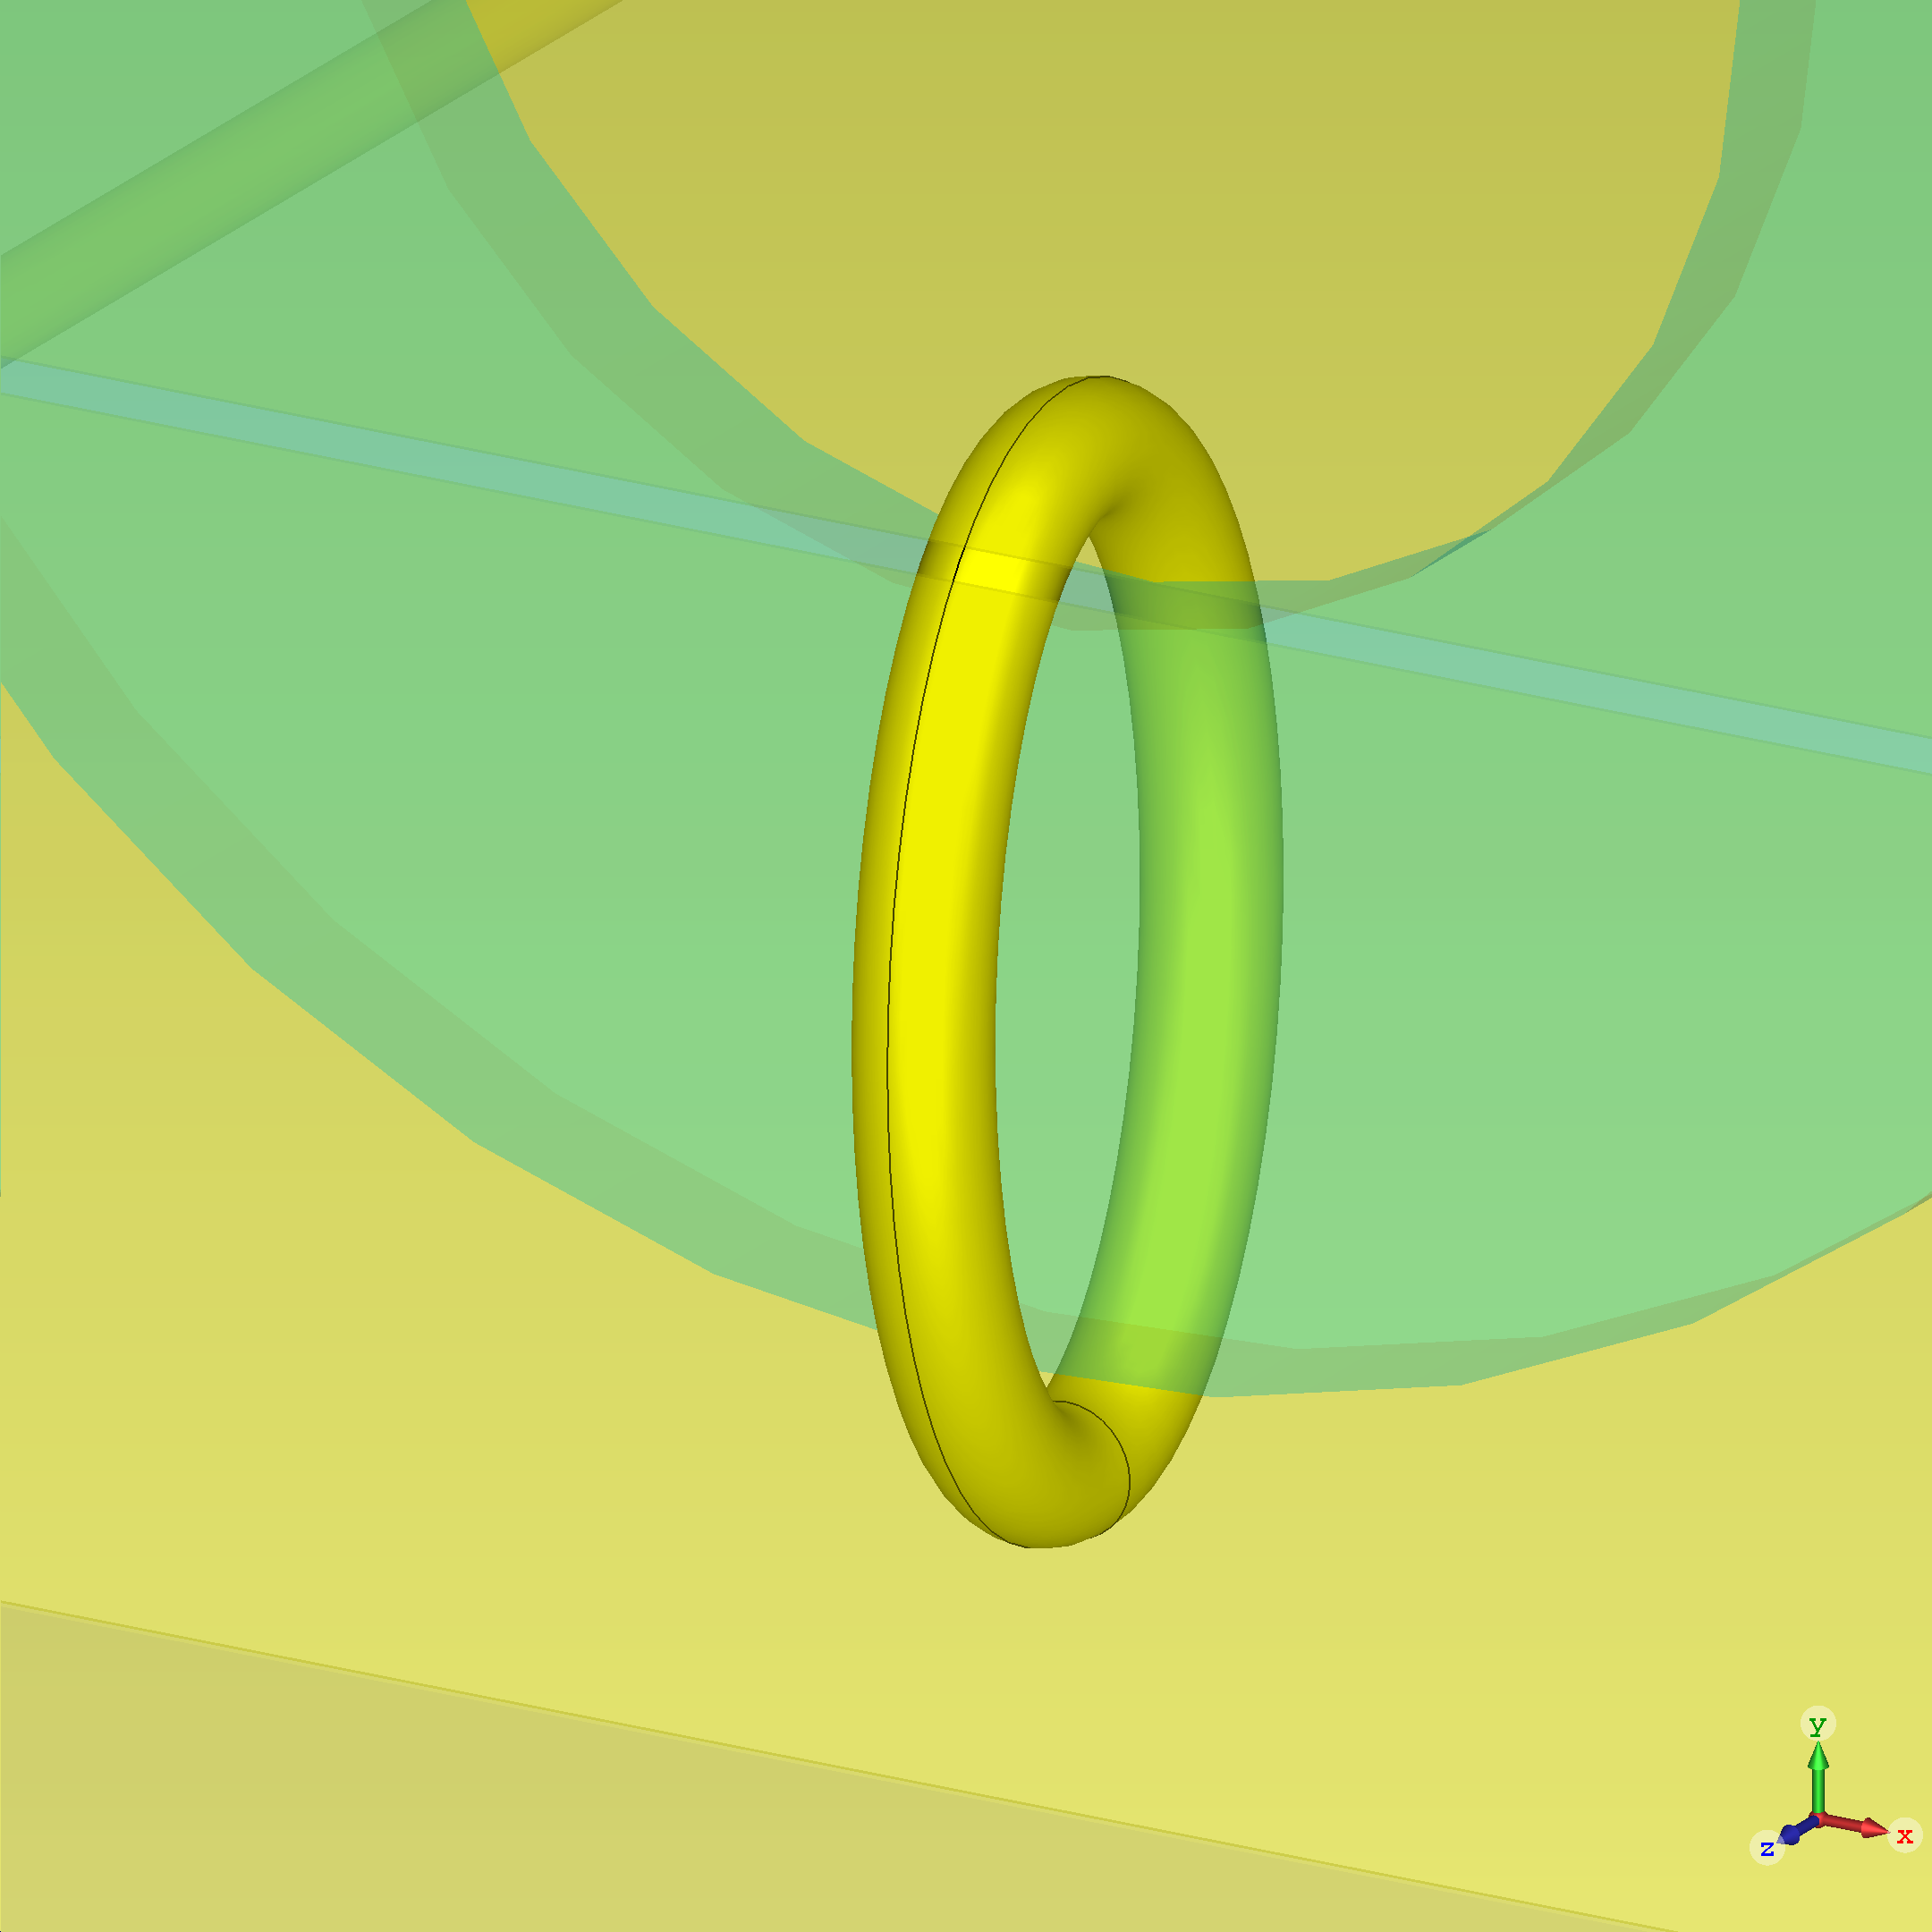
\includegraphics[height=0.3\textwidth]{./Simulation/KSV1Torus.png}}
                \hspace{0.01\textwidth}
                \subfloat[Version 2]{
                    \label{subfig:V2}
                    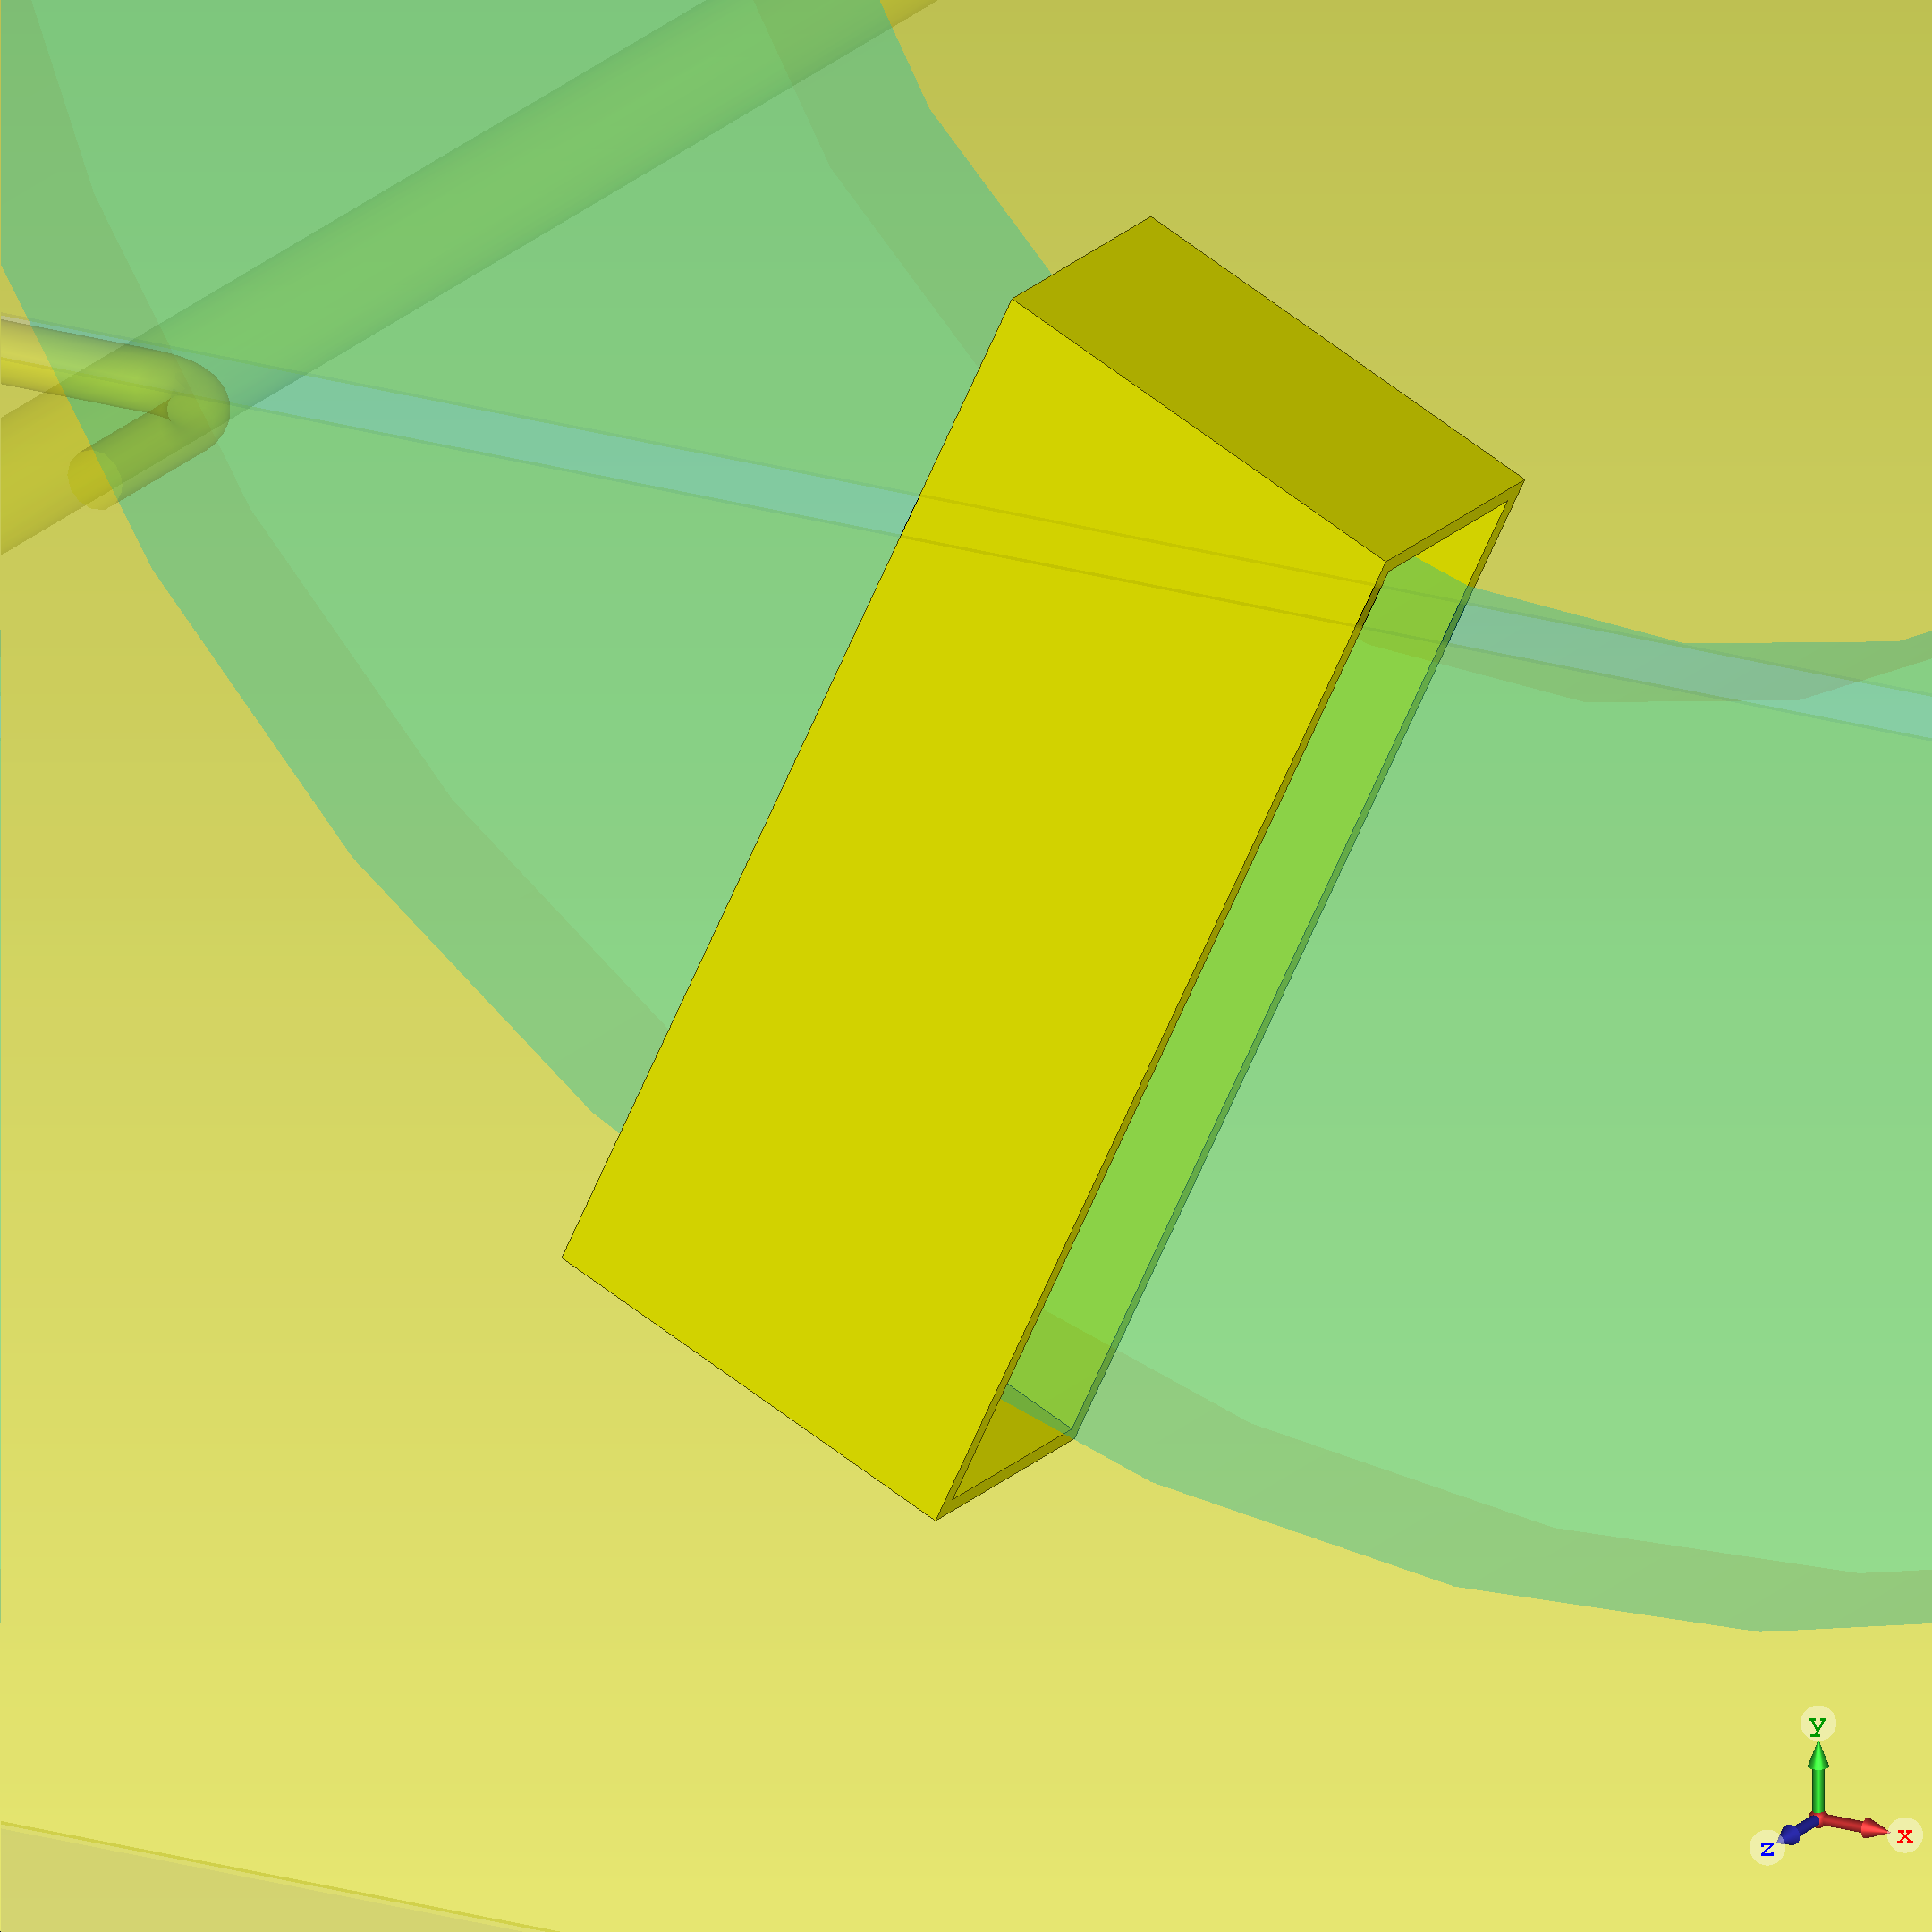
\includegraphics[height=0.3\textwidth]{./Simulation/KSV2Schiene.png}}
                \hspace{0.01\textwidth}
                \subfloat[Version 3]{
                    \label{subfig:V3}
                    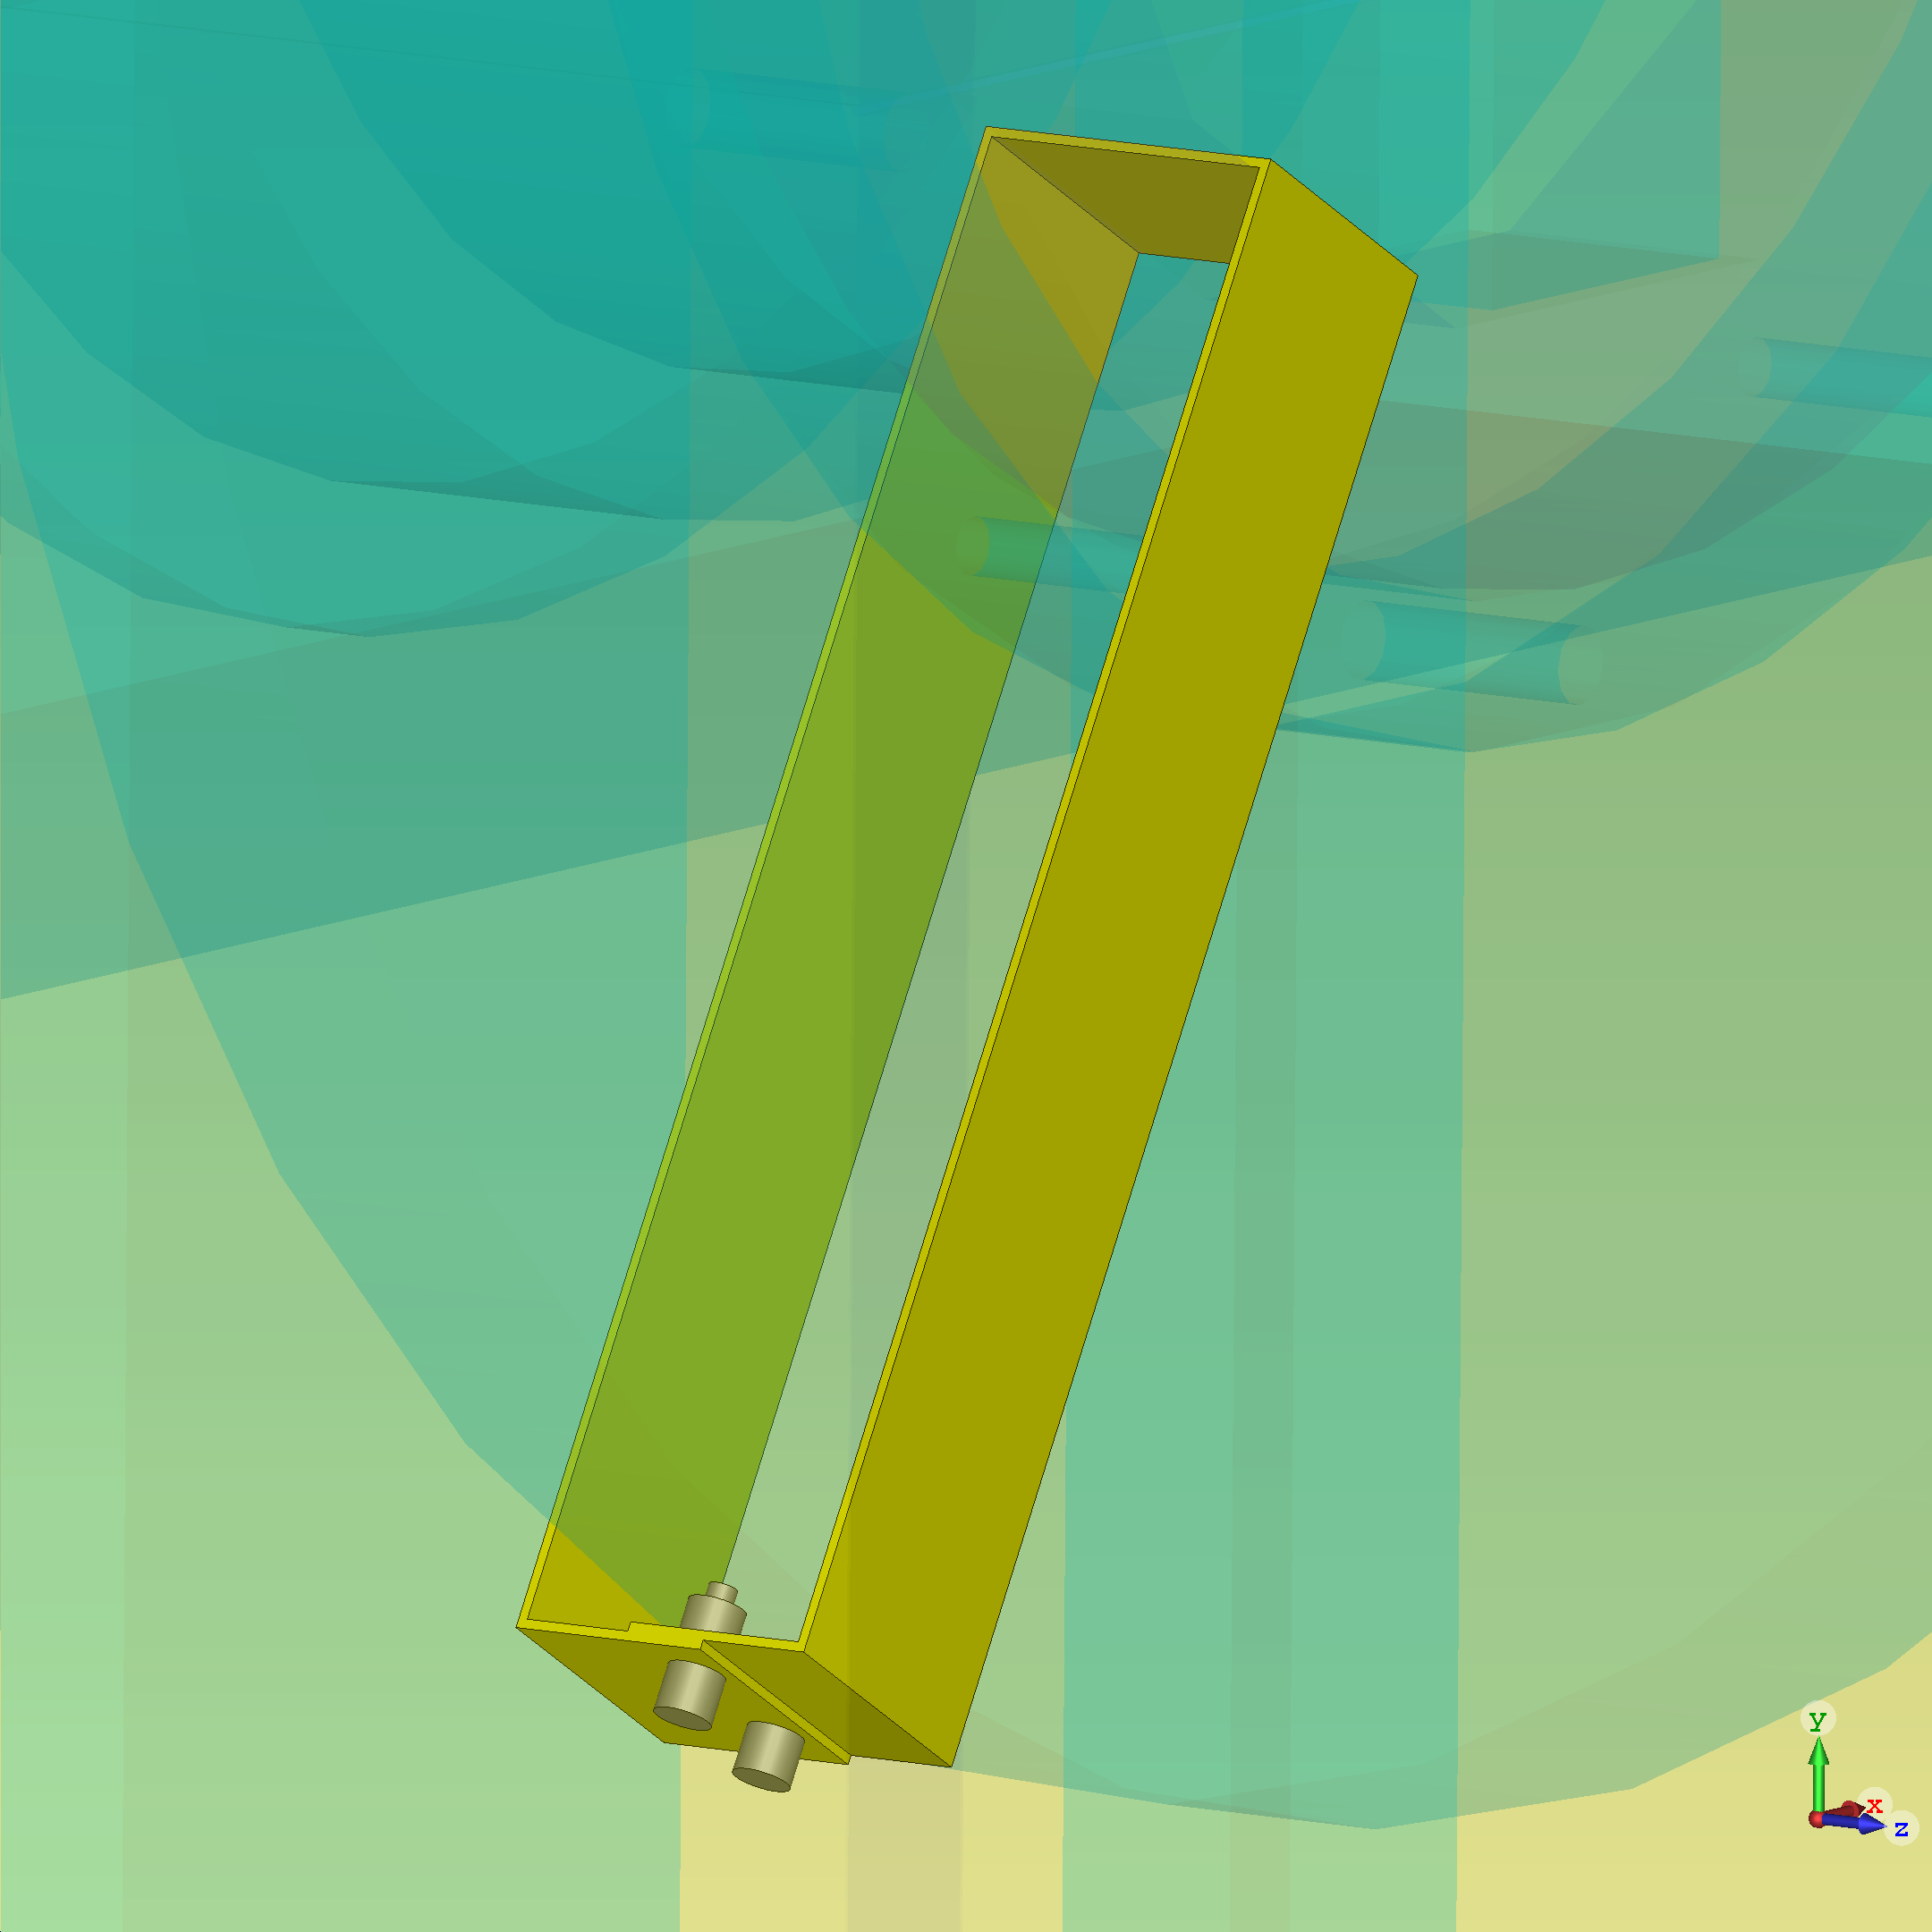
\includegraphics[height=0.3\textwidth]{./Simulation/KSV3MitSchrauben.png}}
                \caption{Modellierung eines Kurzschluss \protect\subref{subfig:V1} als Torus, \protect\subref{subfig:V2} als Schiene und \protect\subref{subfig:V3} in gefertigter Ausführung}
                \label{fig:KSCST}
            \end{figure}
        
        Um eine Parameteranalyse durchzuführen und die Simulationsergebnisse mit den Messungen gegenüberzustellen, ist die finale Version in den verschiedenen Ausführungen, wie sie aus Kapitel~\ref{sec:shorts} hervorgehen, nachgebildet.
        
        \subsection{Realitätsgetreue Anpassungen}
        
        \todo[inline,color=red!30]{Hier weiter ausarbeiten!}
        
        Um das bestehende Testboxmodell und die Simulation noch besser mit der Realität und Messung in Übereinstimmung zu bringen, wurde es um einige Komponenten erweitert.\\
        Das Modell der Testbox wurde um die hölzerne Halterung der Ringkerne ergänzt, da durch die dielektrischen Eigenschaften von Holz ein wenn auch kleiner Einfluss auf die elektrischen Eigenschaften der Testbox zu erwarten ist. Außerdem wurden einige in der Testbox enthaltene Bauteile aus Kupfer hinzugefügt, da diese den Feldverlauf beeinflussen. Dies sind unter anderem ein Bügel, der oberhalb der Einkopplung angebracht ist, sowie eine zylinderförmige Verstärkung am hinteren Ende der Einkopplungsstange.
        
            \subsubsection{Ringkern}
            Auch der Ringkern wurde im Laufe der Arbeit realitätsnäher modelliert.\\
            Dazu wurde wie bereits in der Arbeit von Denys Bast vorgegangen und aus der gemessenen Gesamtimpedanz die verlustbehafteten, magnetischen Materialparameter $\mu'$ und $\mu''$ errechnet und schließlich in CST dem Ringkernmaterial hinzugefügt.\\
            Zu Erst wird über die Impedanzgleichung einer Ersatzschaltungsanordnung für die TEstbox inklusive Ringkern die Impedanz des Ringkerns herausgerechnet. Daraus werden nun die Parameter gewonnen. Diese werden dann in CST den Materialparametern des Ringkerns hinterlegt.
           \todo[inline, color=red!30]{Formeln, Referenz}
           
        \subsection{Erweiterung des Modells}
        Die Testbox wurde im Lauf dieser Arbeit modifiziert, um eine einfacherer Messdurchführung und eine erhöhte Reproduzierbarkeit der Messungen zu erreichen, diese Modifikationen wurden auch in die Simulationsmodellierung übernommen.\\
        Die Ringkernhalterung wurde um das Holzkreuz ergänzt und der Polygonzug zur Befestigung der Kurzschlüsse wurde geometrisch exakt eingefügt.\\
        
        \sout{Dieser Text soll nicht sein.}\textcolor{red}{Dieser Schon.}

